\chapter{All-sky Analysis}
\label{sec:analysis}

    We inspect the IR abd AME data in 3 approaches, relying on HEALPix maps at ~1$^{\circ}$ angular resolution. We start with an all-sky AME to IR comparison, looking for global patterns among all pixels (except those within 10$^{\circ}$ of the ecliptic plane.) 2) Next we show a more regionalized comparison, looking at the set of AME-prominent galactic clouds identified by the \cite{planckXV}. As much as possible, we maintain comparability between their IRAS-Planck based result, and our result which adds-in AKARI data and dust SED fitting. 3) Lastly, we highlight the $\lambda$~Orionis molecular ring \citep{maddalena86,maddalena87}, a particular AME-dominated region with resolvable structure even at ~1$^{\circ}$ angular resolution.

\section{All-sky Pixel Domain Analysis}

	In order to look more closely at the variations between the individual bands' maps, we include a pixel-by-pixel analysis. Figure \ref{fig:AMEvsDust_allsky_allbands} shows the result of such a comparison, for each of the 18 bands sampled. The AME data comes from the PR2 AME map.

    To keep our analysis comparable to previous works, we exclude pixels within 10$^{\circ}$ of the ecliptic plane, where the Zodi-residuals can be a problematic (especially in the MIR.)

     Figure \ref{fig:AME_IR_crosscorr_allbandsg} visualizes the cross-correlation matrix for each of the IR bands. The AME does not show a strong correlation with other bands at $|l|>10$. At $|l|<10$, the FIR bands show stronger correlation. The PAH-tracing bands show a stronger correlation than bands at 18 to 60~$\mu$m, but weaker than AME vs. the FIR bands.

  To understand how these trends may vary across the sky, we repeat the correlation analysis along 1$^{\circ}$ width latitude strips. For each degree of $b$, we cross correlate the Planck modified blackbody fitting results vs. the AME and the AKARI 9~$\mu$m intensity. (This comes with the geometrical caveat that the higher latitude bins have fewer samples.) The results of this comparison are shown in \ref{fig:PlanckModBBvsAMEandA9_bins}. Fig. \ref{fig:PlanckModBBvsAMEandA9_bins}) shows the result with longitude strips. The $l$ based comparison produces a consistent ranking of the correlation strengths all longitudes. There is an unexplained variation between $b = 200$ and 250.

  Finally, we produce an all-sky correlation map. From the NSIDE 256 input maps of each of dust temperature $T$, radiance $R$, and emissivity index beta, and $I 9~\mu$m, we produce NSIDE 16 maps of $S$ for correlation strength vs. AME. These maps are shown in Fig. \ref{fig:Spearman_Map_nside16_AMEtoMBBandA9}.

      \begin{figure*}
        \label{fig:AME_IR_crosscorr_allbandsg}
        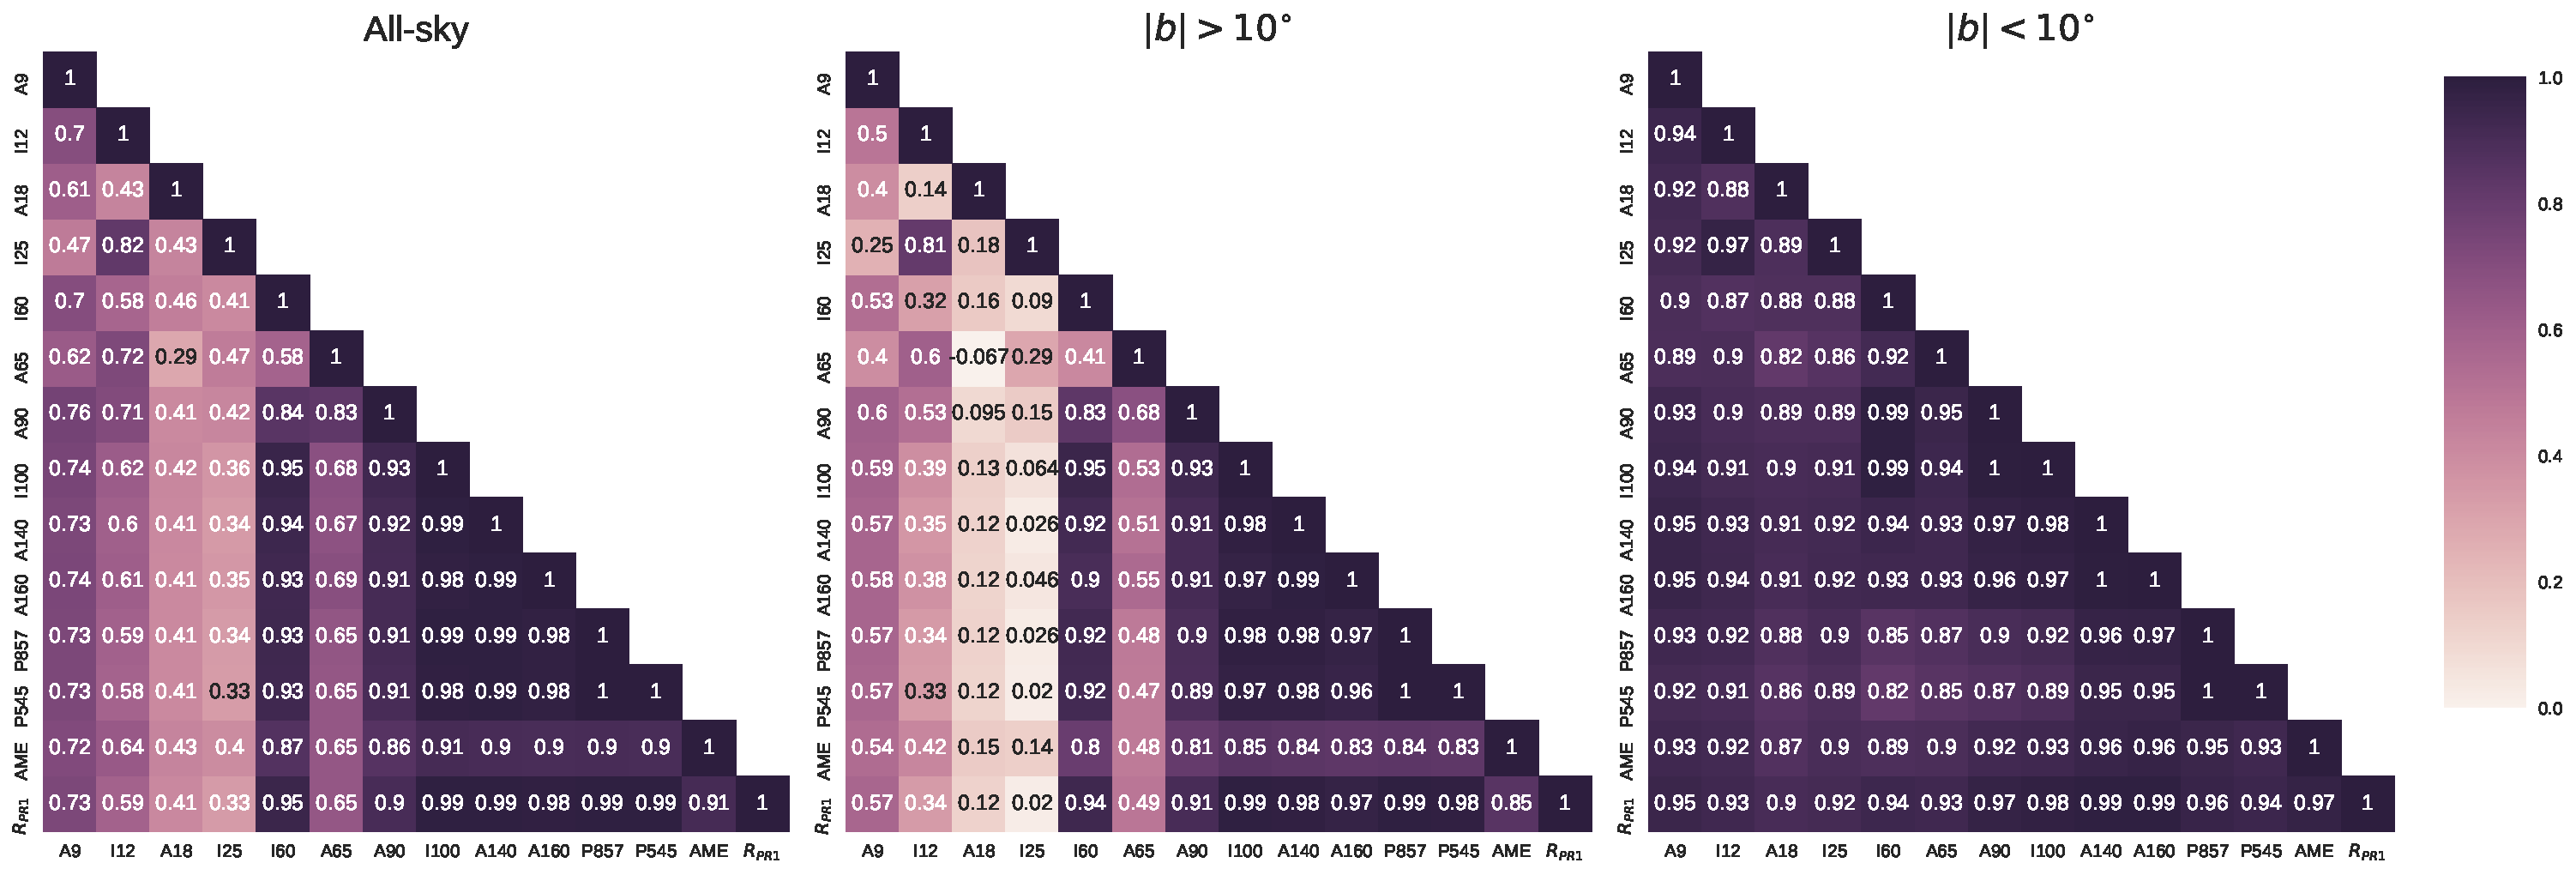
\includegraphics[width=185mm]{../Plots/all_bands_corr_matrix_wAME_spearman.pdf}
        \centering
        \caption{ALL-SKY cross-correlation matrix for the 18 infrared bands sampled, and the AME map. THe color-scale indicates the Spearman rank ($S$). Results are based on the full sky (excluding pixels within 10$^{\circ}$ of the ecliptic plane).}
      \end{figure*}

      \begin{figure*}
        \label{fig:AMEvsDust_allsky_allbands}
        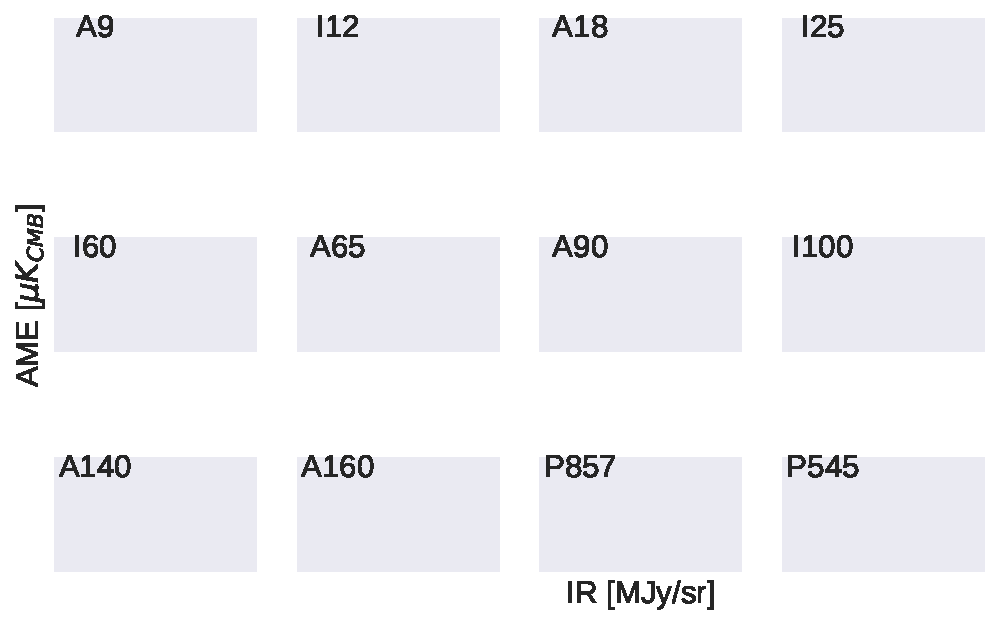
\includegraphics[width=150mm]{../Plots/AMEvsDust_allsky_allbands.pdf}
        \centering
        \caption{ALL-SKY kernel density estimates of 12-band infrared photometry against the PR2 AME map. Pixels within 10$^{\circ}$ of the ecliptic plane are excluded. 'A' indicates AKARI; 'D', DIRBE; 'I', IRAS, and 'P' Planck. The number after each letter indicates the band central nominal wavelength in microns (or frequency in GHz, in the case of the Planck bands.) }
      \end{figure*}

      \begin{figure*}
        \label{fig:AMEtoRvsDusttoR_allsky_allbands}
        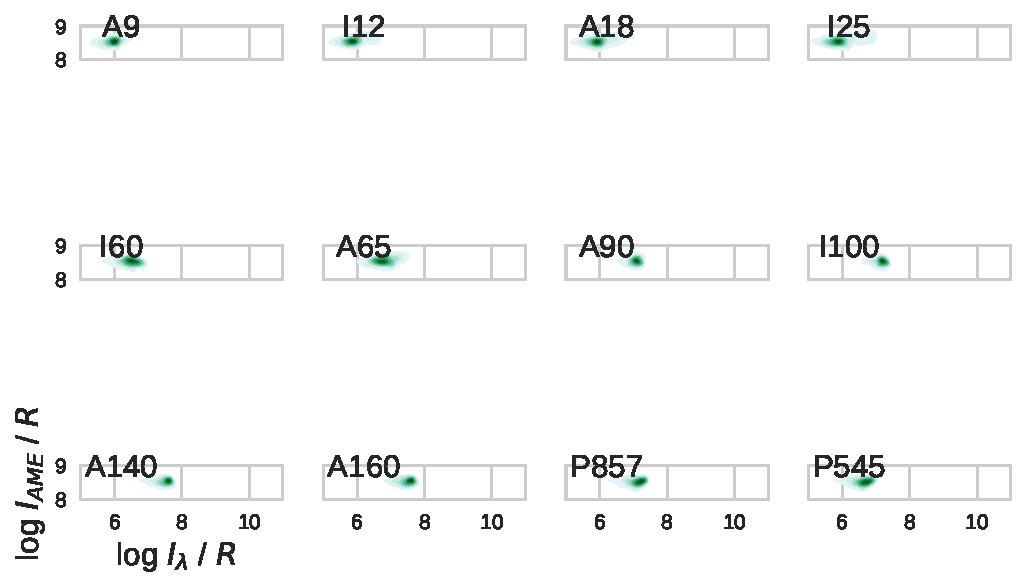
\includegraphics[width=150mm]{../Plots/AMEvsDust_allsky_allbands__mpsub_Rnorm_kde.pdf}
        \centering
        \caption{Similar comparison to Fig. \ref{fig:AMEvsDust_allsky_allbands}, with both the IR and the AME intensities scaled by the PR2 dust radiance ($R$) for each pixel. }
      \end{figure*}

      \begin{figure*}
        \label{fig:Spearman_Map_nside8_AMEto}
        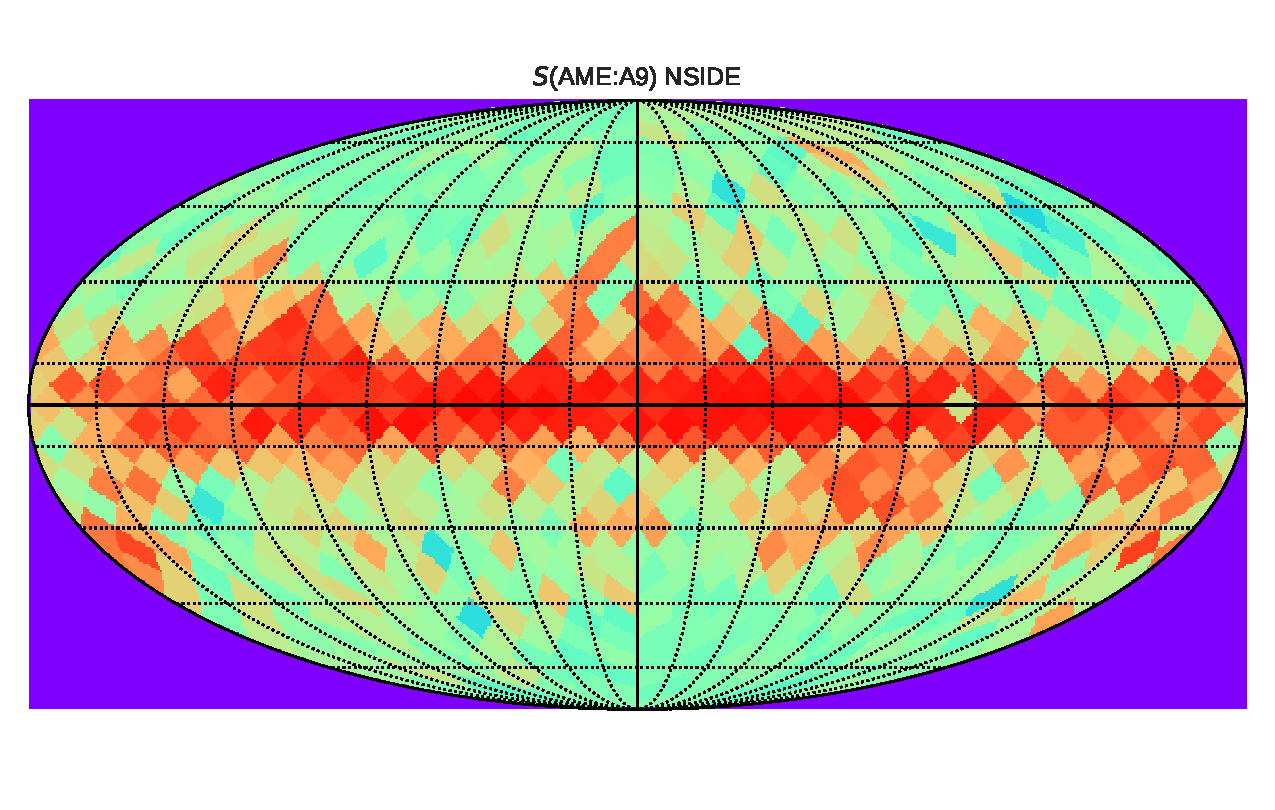
\includegraphics[width=80mm]{../Plots/Allsky_Corr/Spearman_Map_nside8_AMEtoA9.pdf}
        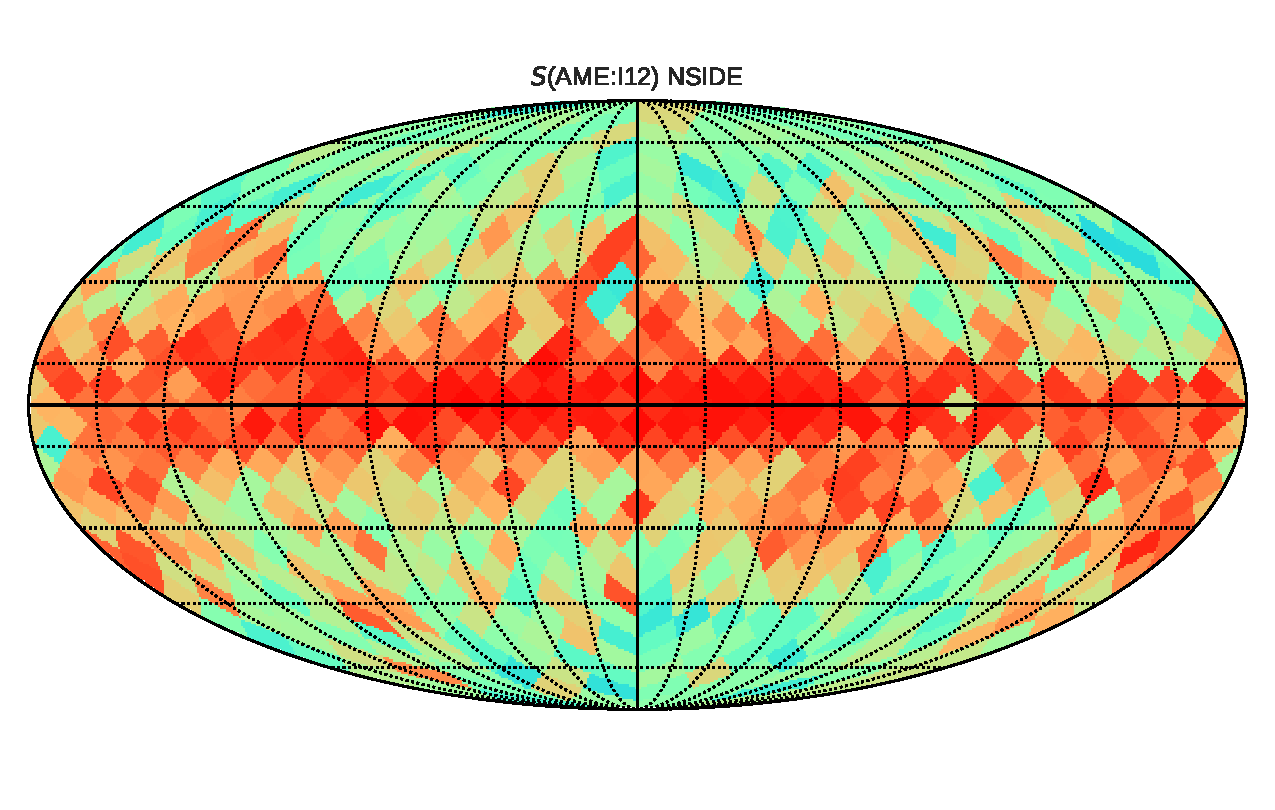
\includegraphics[width=80mm]{../Plots/Allsky_Corr/Spearman_Map_nside8_AMEtoI12.pdf}
        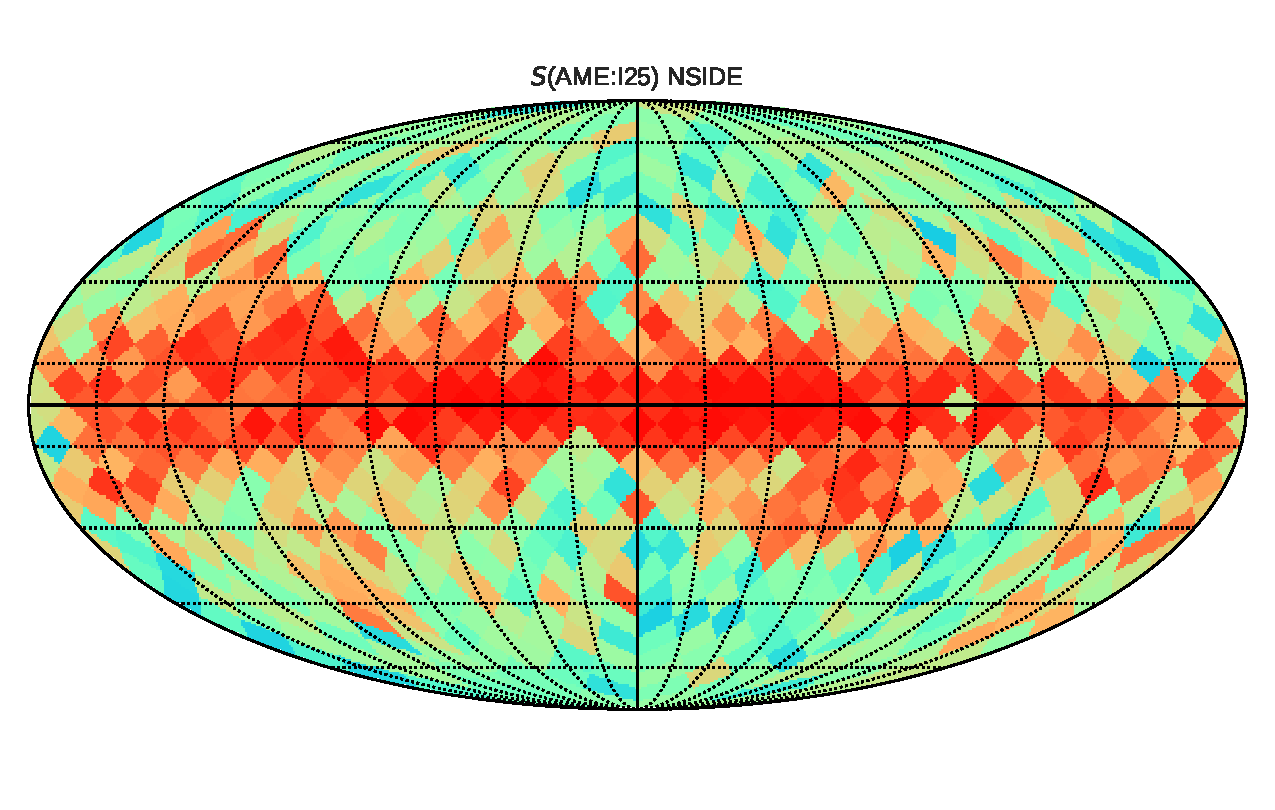
\includegraphics[width=80mm]{../Plots/Allsky_Corr/Spearman_Map_nside8_AMEtoI25.pdf}
        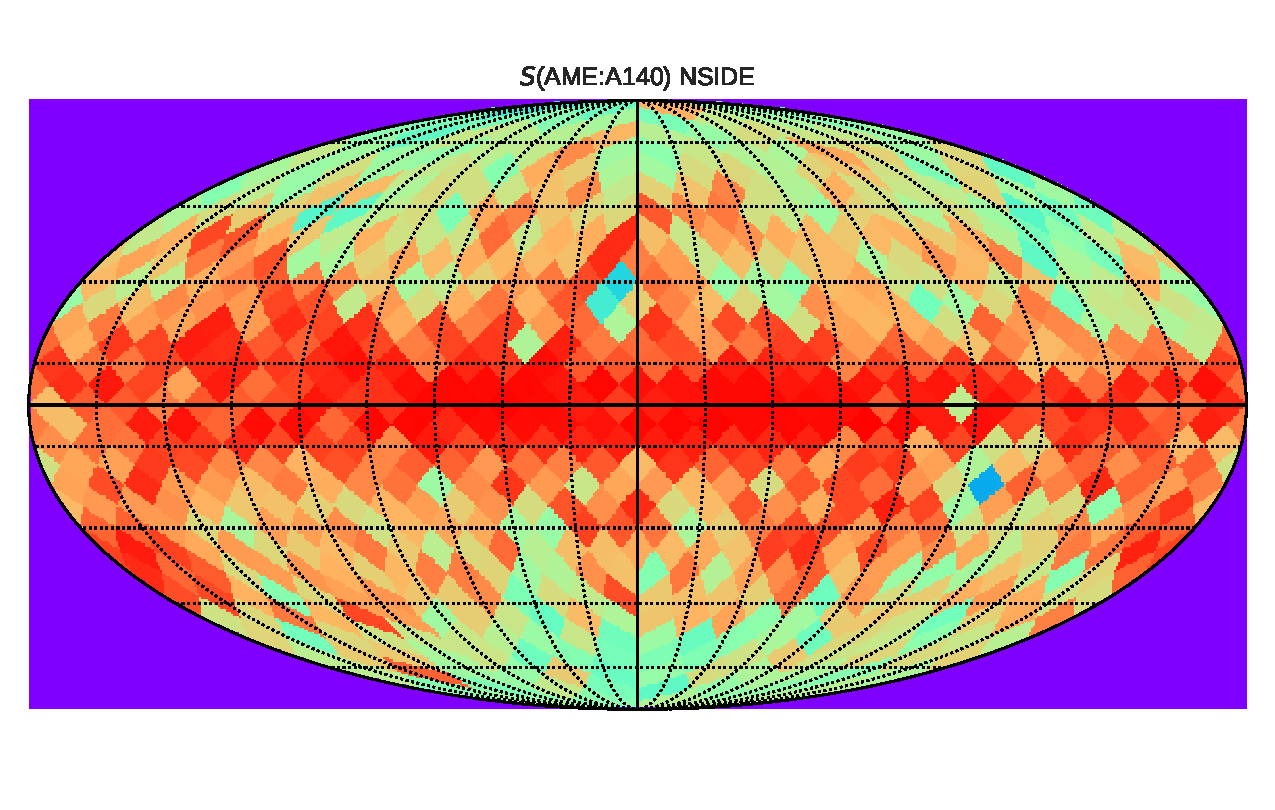
\includegraphics[width=80mm]{../Plots/Allsky_Corr/Spearman_Map_nside8_AMEtoA140.pdf}
        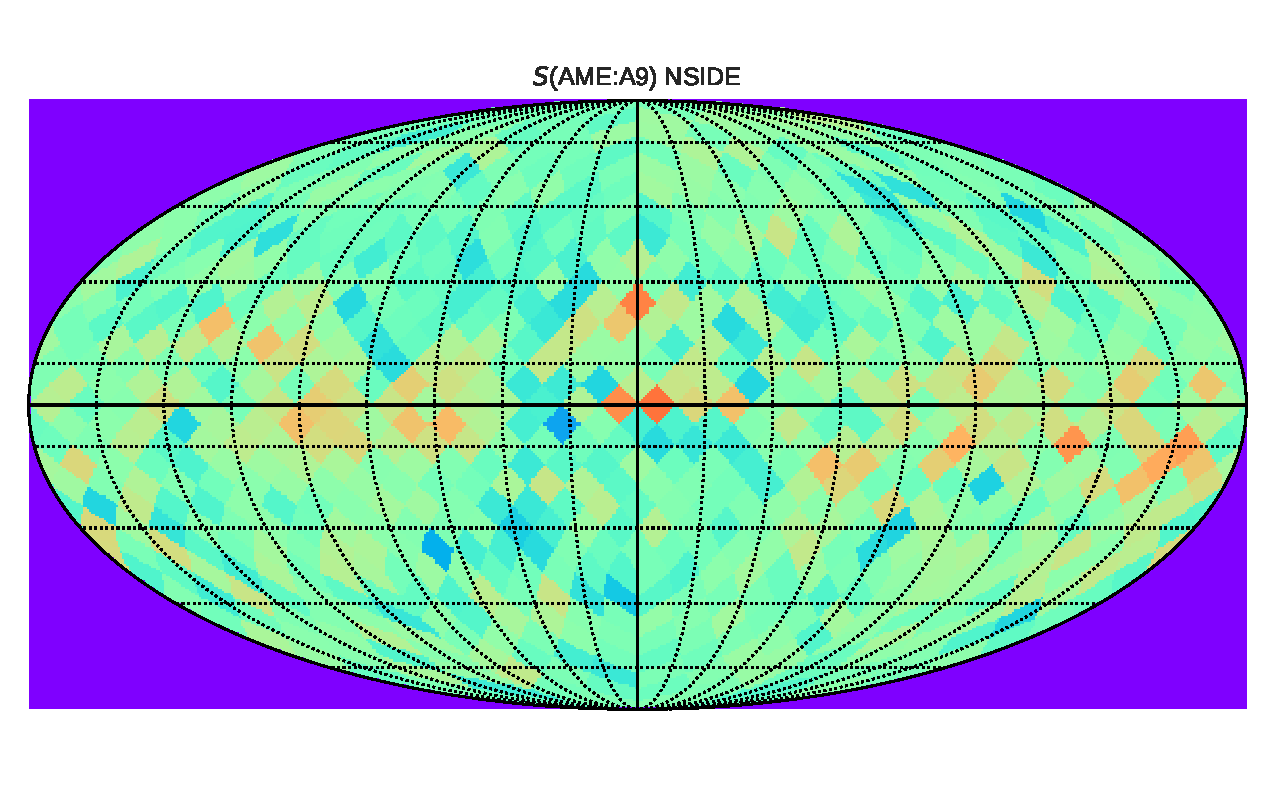
\includegraphics[width=80mm]{../Plots/Allsky_Corr/RadNorm/Spearman_Map_nside8_AMEtoA9.pdf}
        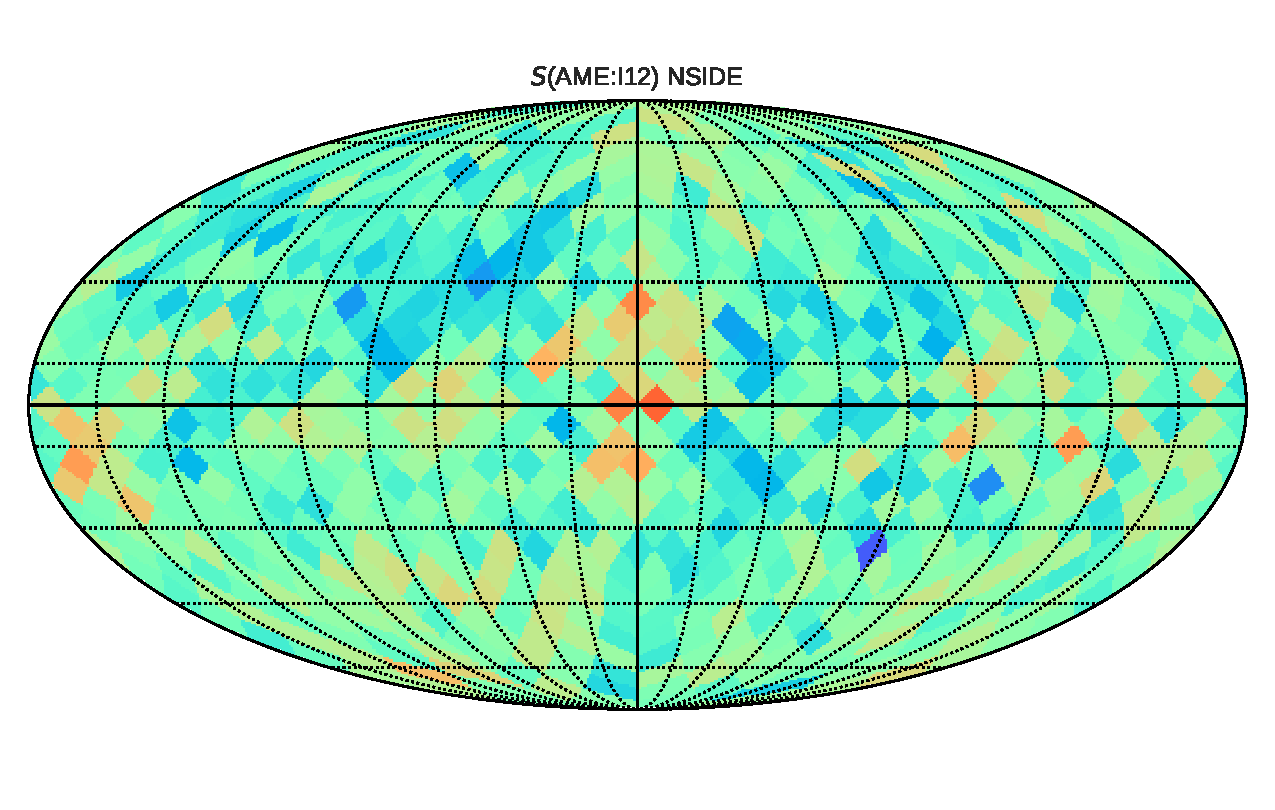
\includegraphics[width=80mm]{../Plots/Allsky_Corr/RadNorm/Spearman_Map_nside8_AMEtoI12.pdf}
        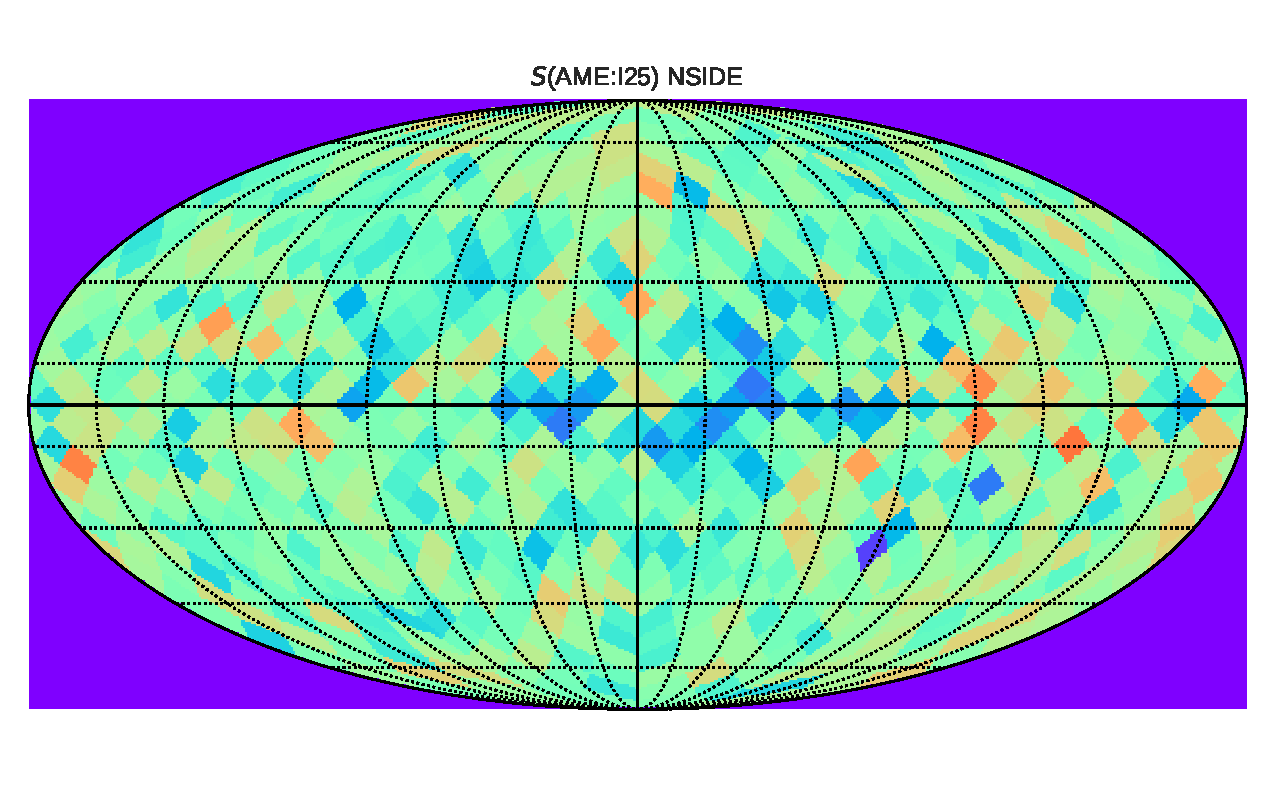
\includegraphics[width=80mm]{../Plots/Allsky_Corr/RadNorm/Spearman_Map_nside8_AMEtoI25.pdf}
        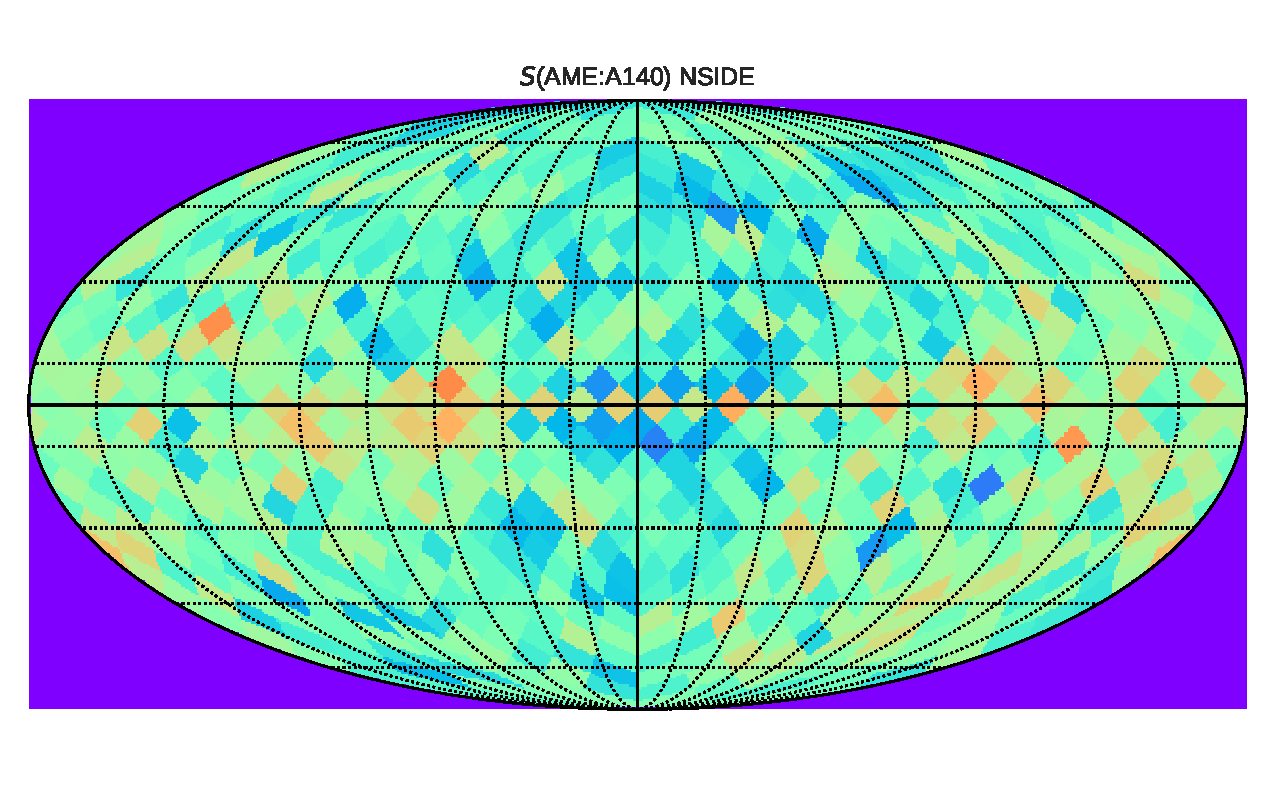
\includegraphics[width=80mm]{../Plots/Allsky_Corr/RadNorm/Spearman_Map_nside8_AMEtoA140.pdf}
        \centering
        \caption{Spatial map of Spearman correlation coefficients between the AME and IR intensity for 4 bands:$9~\mu{}m$, $12~\mu{}m$, $25~\mu{}m$, and $140~\mu{}m$. $S$ is calculated for all NSIDE 256 pixels within each NSIDE 8 pixel-sized bin.}
      \end{figure*}
